\subsection{Branches and Tags}
\renewcommand{\figurename}{Diagram}

Technically Subversion does not introduce separate concepts for branches and tags. Both branches and tags are versioned directories under repository root. As result Translator performs theirs translation in similar way. There are differences at Git level only:
\begin{enumerate}
	\compactlist
	\item Addition.
	\begin{itemize}
		\item Creation of /branches/\emph{B} directory leads to creation of a new branch reference \emph{B}.
		\item Creation of /tags/\emph{T} directory leads to addition of corresponding Tag Object with name \emph{T}.
	\end{itemize}
	\item Modification.
	\begin{itemize}
		\item Change at /branches/\emph{B} directory leads to updating of corresponding branch reference \emph{B}.
		\item Change at /tags/\emph{T} directory leads to the removal of obsolete Tag Object with name \emph{T} and creation of new Tag Object with the same name for corresponding Commit Object.
	\end{itemize}
	\item Deletion.
	\begin{itemize}
		\item Removal of /branches/\emph{B} directory leads to removal of corresponding reference \emph{B} at Git repository, when
		\item Removal of /tags/\emph{T} directory leads to removal of corresponding Tag Object with name \emph{T}.
	\end{itemize}
\end{enumerate}

The same rules could be treated in opposite direction --- every change of Git branch or tag leads to corresponding change of Subversion branch or tag.
\\\\
This and further chapters consider scenarios with branches only. Every scenario could be applied to tags with the rules above taken into account.
\\\\
Basically Translator tracks all the references located at Git repository and synchronizes every such reference with certain Subversion branch. The exact way of this synchronization described further.

\subsubsection{Creation}

There is a couple of ways to create branch in Subversion keeping history of another branch (or the same branch from certain revision):
\\\\
1. Branch creation by copying, see diagram \ref{branch_creation_svn_to_git}.
\begin{center}
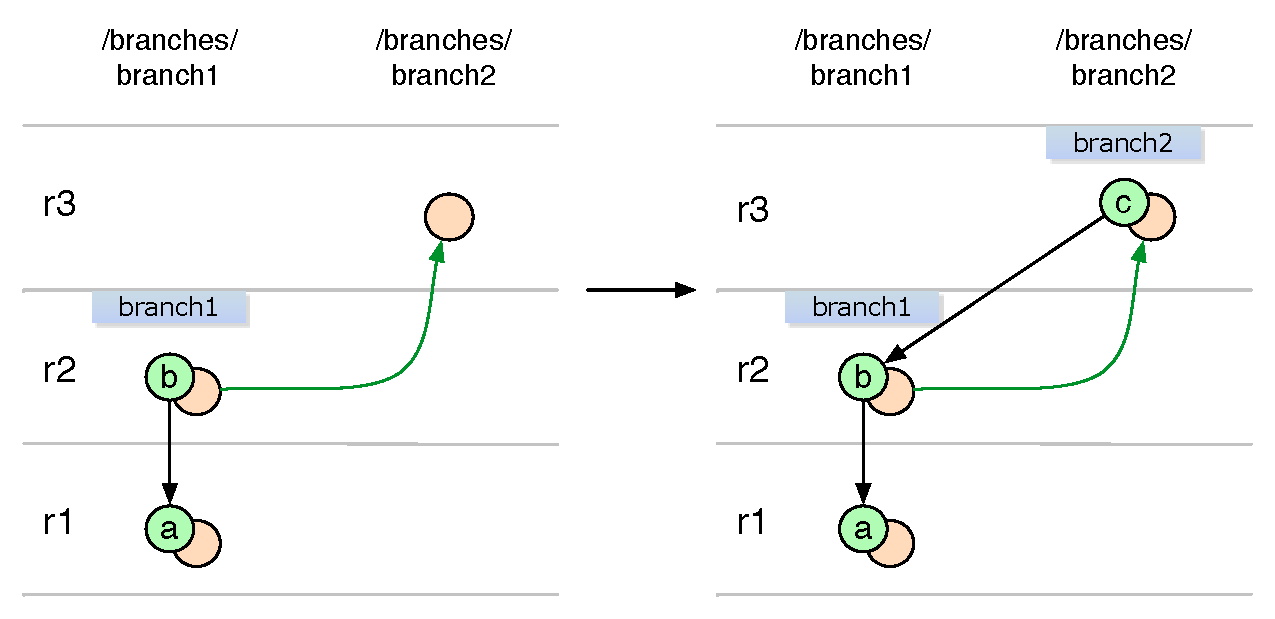
\includegraphics[width=\textwidth]{img/diagrams/branch_creation_svn_to_git.pdf}%
\captionof{figure}{Subversion branch copy being translated to Git branch creation.}
\label{branch_creation_svn_to_git}%
\end{center}

2. Branch creation with merge history, see diagram \ref{branch_creation_from_mergeinfo_svn_to_git}.
\begin{center}
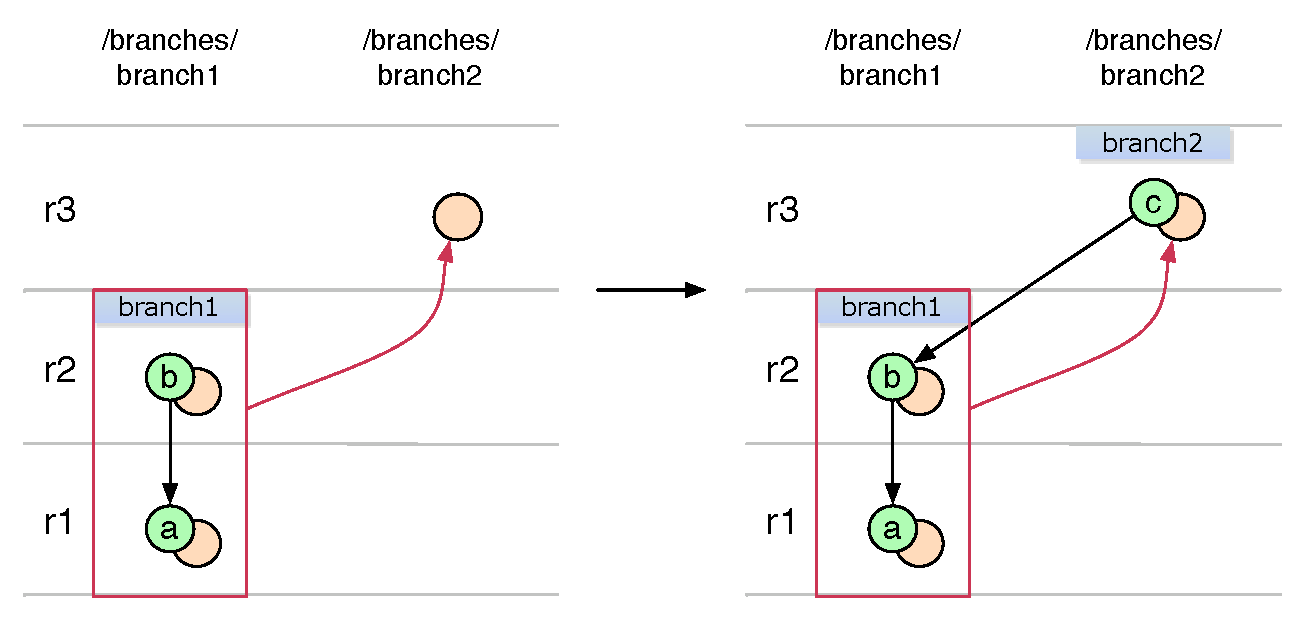
\includegraphics[width=\textwidth]{img/diagrams/branch_creation_from_mergeinfo_svn_to_git.pdf}%
\captionof{figure}{Subversion branch addition with merge history being translated to Git branch creation.}
\label{branch_creation_from_mergeinfo_svn_to_git}%
\end{center}

Git to Subversion translation behaves as depicted at diagram \ref{branch_creation_git_to_svn}.
\begin{center}
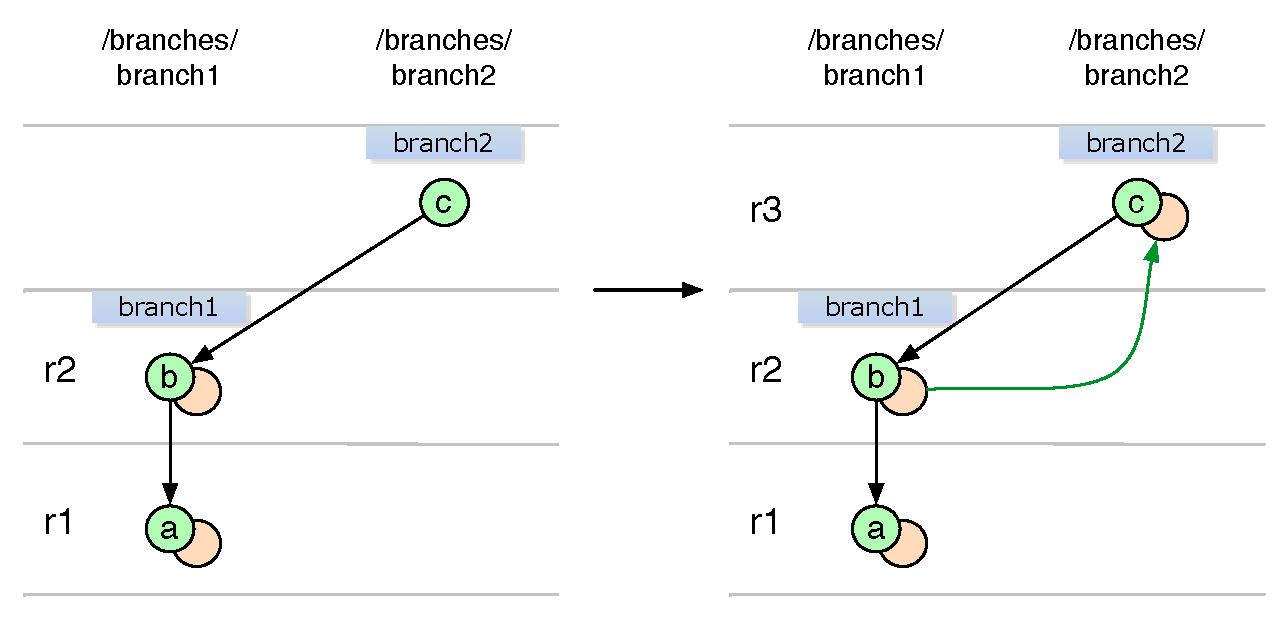
\includegraphics[width=\textwidth]{img/diagrams/branch_creation_git_to_svn.pdf}%
\captionof{figure}{Git branch addition being translated to Subversion branch copy.}
\label{branch_creation_git_to_svn}%
\end{center}

Branches could also be created with no history. This kind of Subversion to Git translation depicted at diagram \ref{branch_creation_no_history_svn_to_git} and corresponding Git to Subversion translation depicted at diagram \ref{branch_creation_no_history_git_to_svn}.

\begin{center}
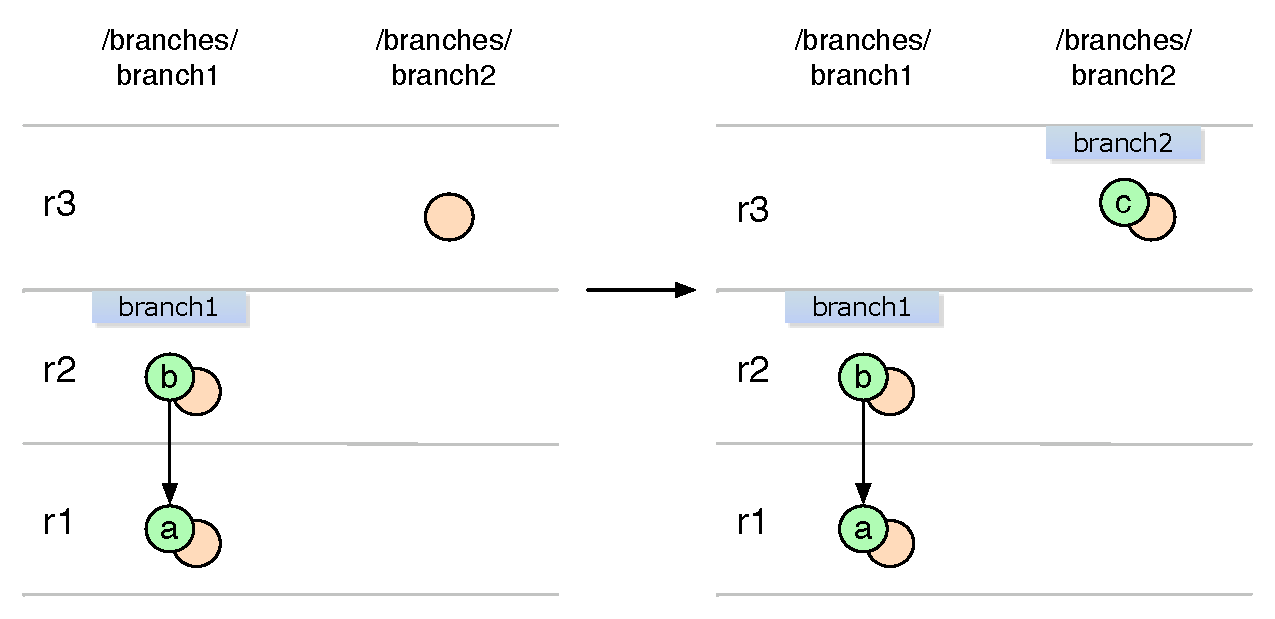
\includegraphics[width=\textwidth]{img/diagrams/branch_creation_no_history_svn_to_git.pdf}%
\captionof{figure}{Subversion branch addition with no history being translated to creation of Git branch referenced to commit with no parents.}
\label{branch_creation_no_history_svn_to_git}%
\end{center}

\begin{center}
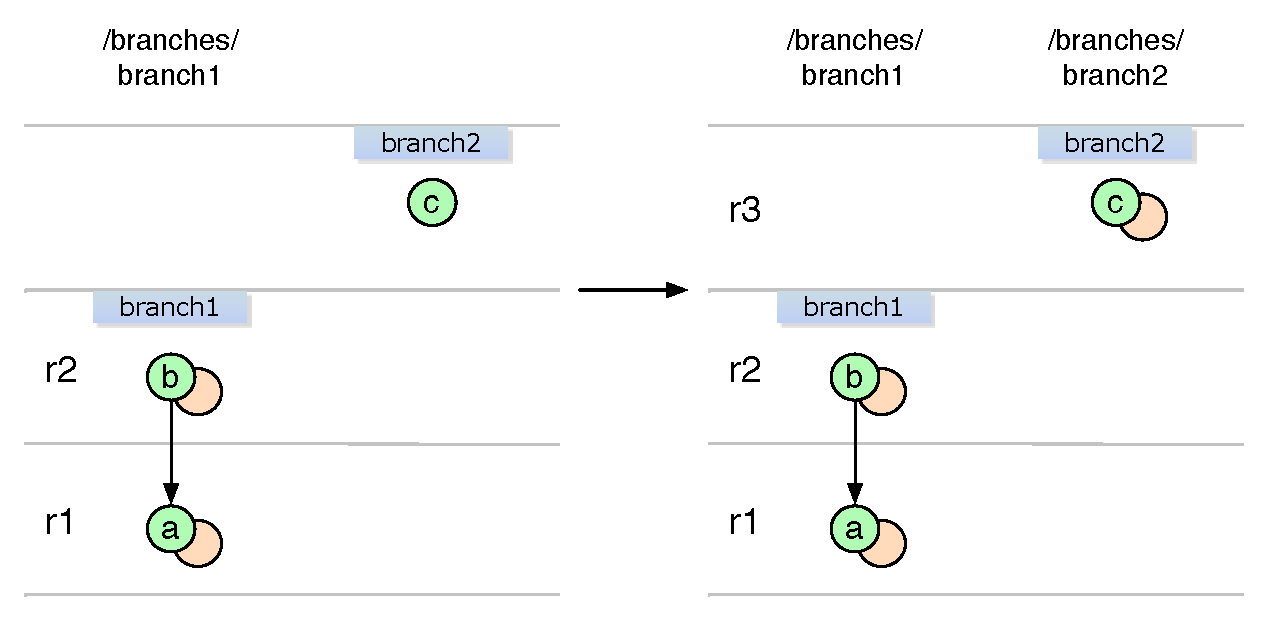
\includegraphics[width=\textwidth]{img/diagrams/branch_creation_no_history_git_to_svn.pdf}%
\captionof{figure}{Addition of Git branch referenced to commit with no parents being translated to Subversion branch creation.}
\label{branch_creation_no_history_git_to_svn}%
\end{center}

Translator always tracks all Git branch references, so addition of such a reference with no commits on the branch is always translated as creation of Subversion branch with no changes. This case depicted at diagram \ref{svn_no_change_branch_creation_git_to_svn}.
\begin{center}
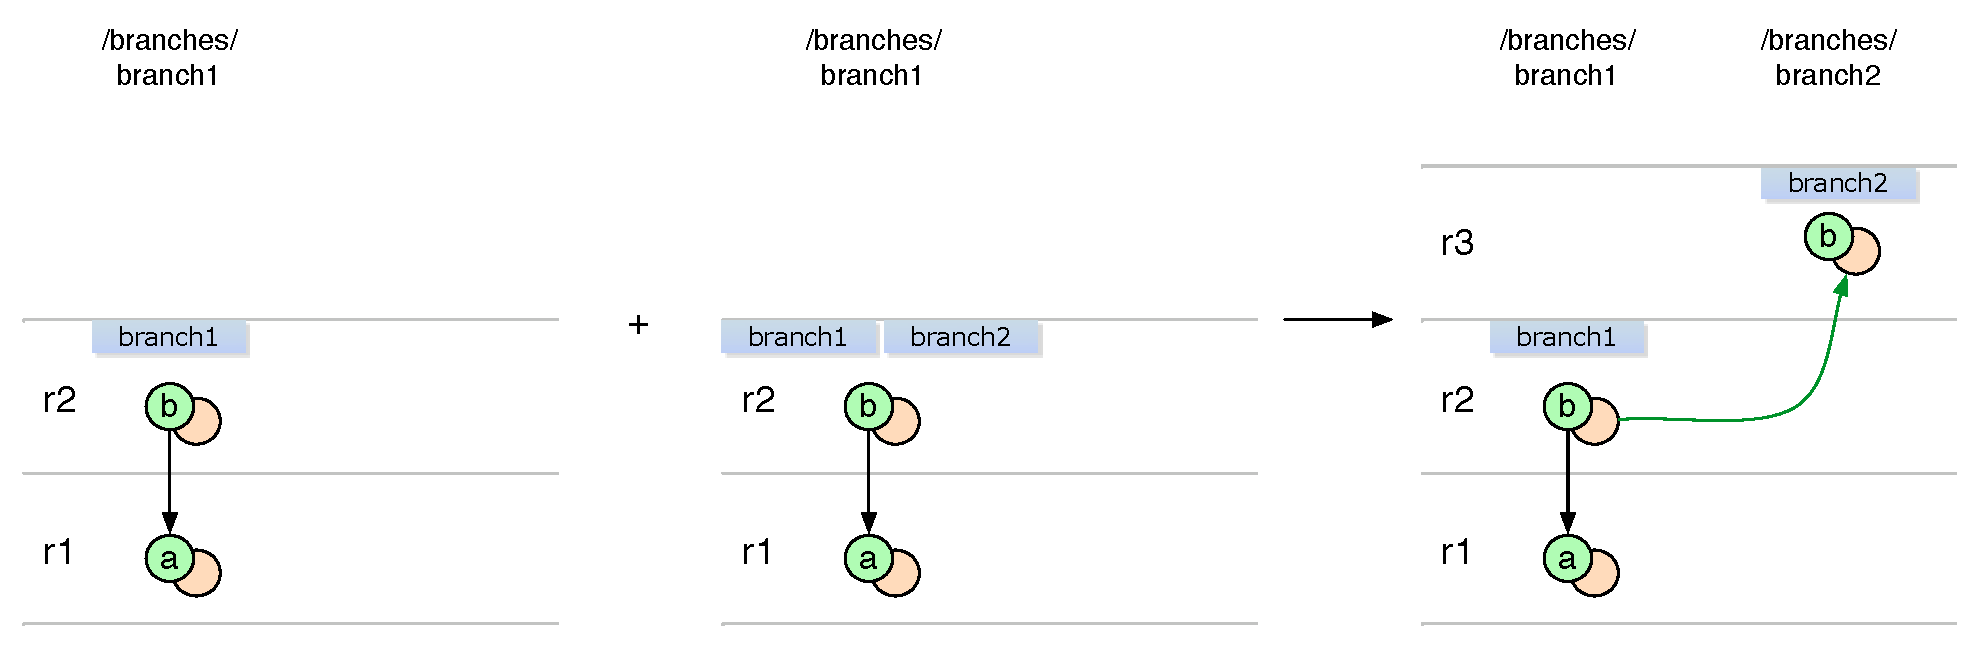
\includegraphics[width=\textwidth]{img/diagrams/svn_no_change_branch_creation_git_to_svn.pdf}%
\captionof{figure}{Addition of second reference to Git commit being translated to creation of Subversion branch with no changes.}
\label{svn_no_change_branch_creation_git_to_svn}%
\end{center}

Revision r3 has synthetically generated commit message and synchronization time as time when revision was created.

\subsubsection{Modification}

The most typical scenarios of branch modification depicted at diagrams \ref{single_change_svn_to_git} and \ref{single_change_git_to_svn}. There are also the following use cases:
\\\\
1. Git user created commit and set two references to it. See diagram \ref{ambiguous_svn_branch_git_to_svn}.
\begin{center}
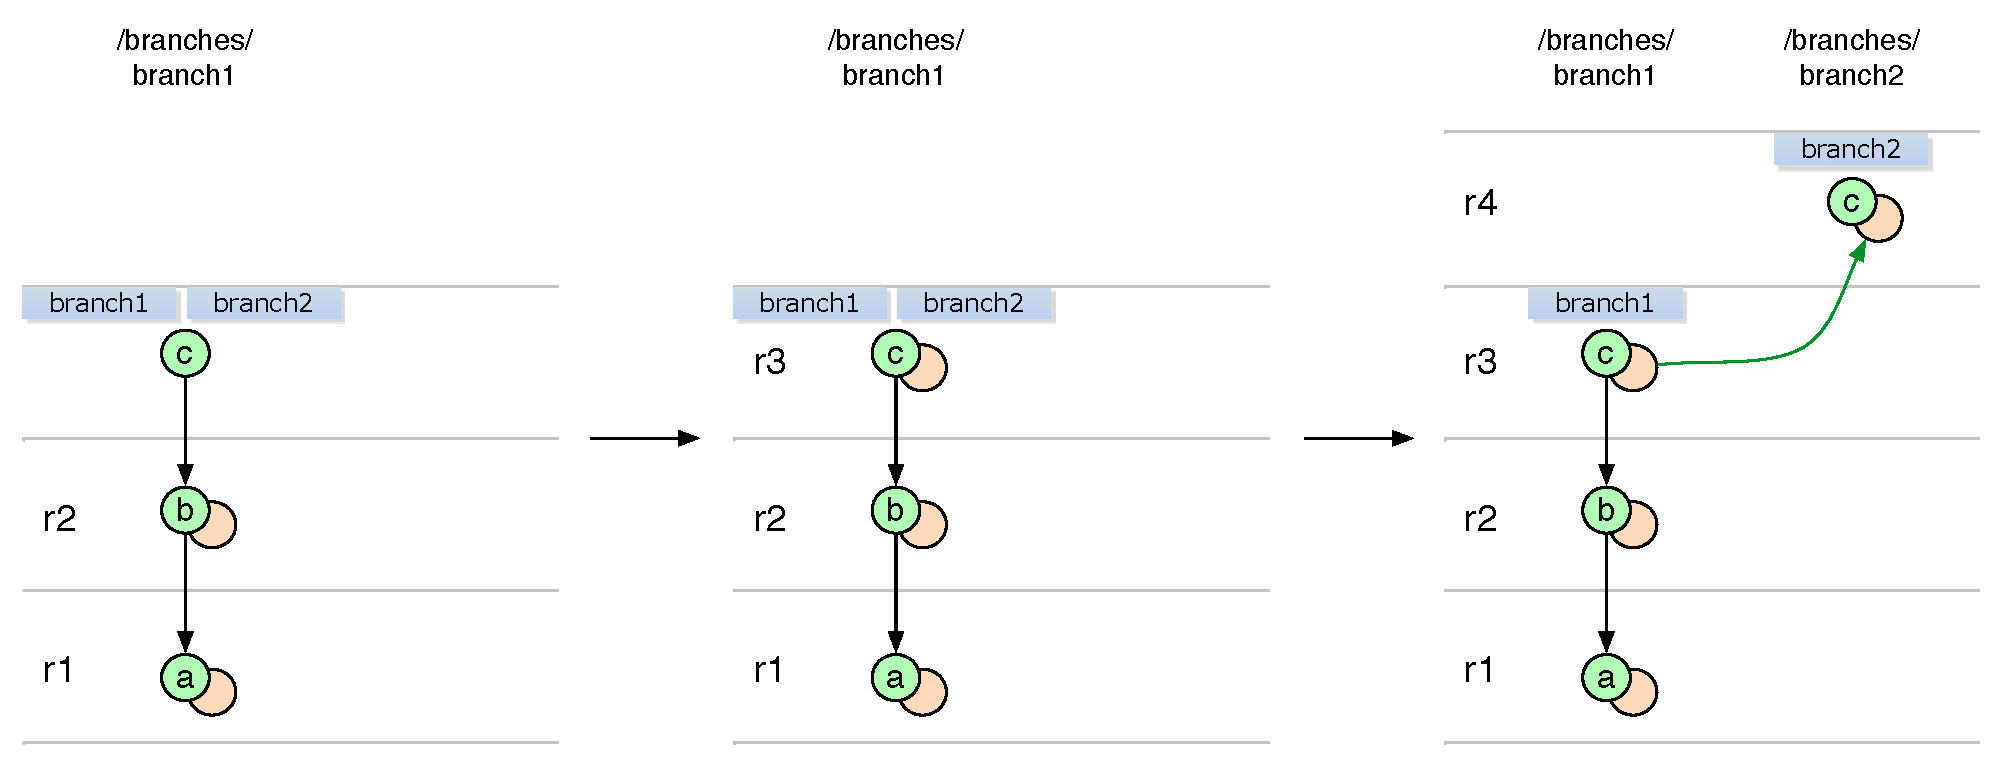
\includegraphics[width=\textwidth]{img/diagrams/ambiguous_svn_branch_git_to_svn.pdf}%
\captionof{figure}{Commit referenced by two branches being translated to Subversion two revisions: modification revision r3 and second branch creation revision r4.}
\label{ambiguous_svn_branch_git_to_svn}%
\end{center}

2. Subversion user modified two branches at a single revision. See diagram \ref{double_branch_change_svn_to_git}.
\begin{center}
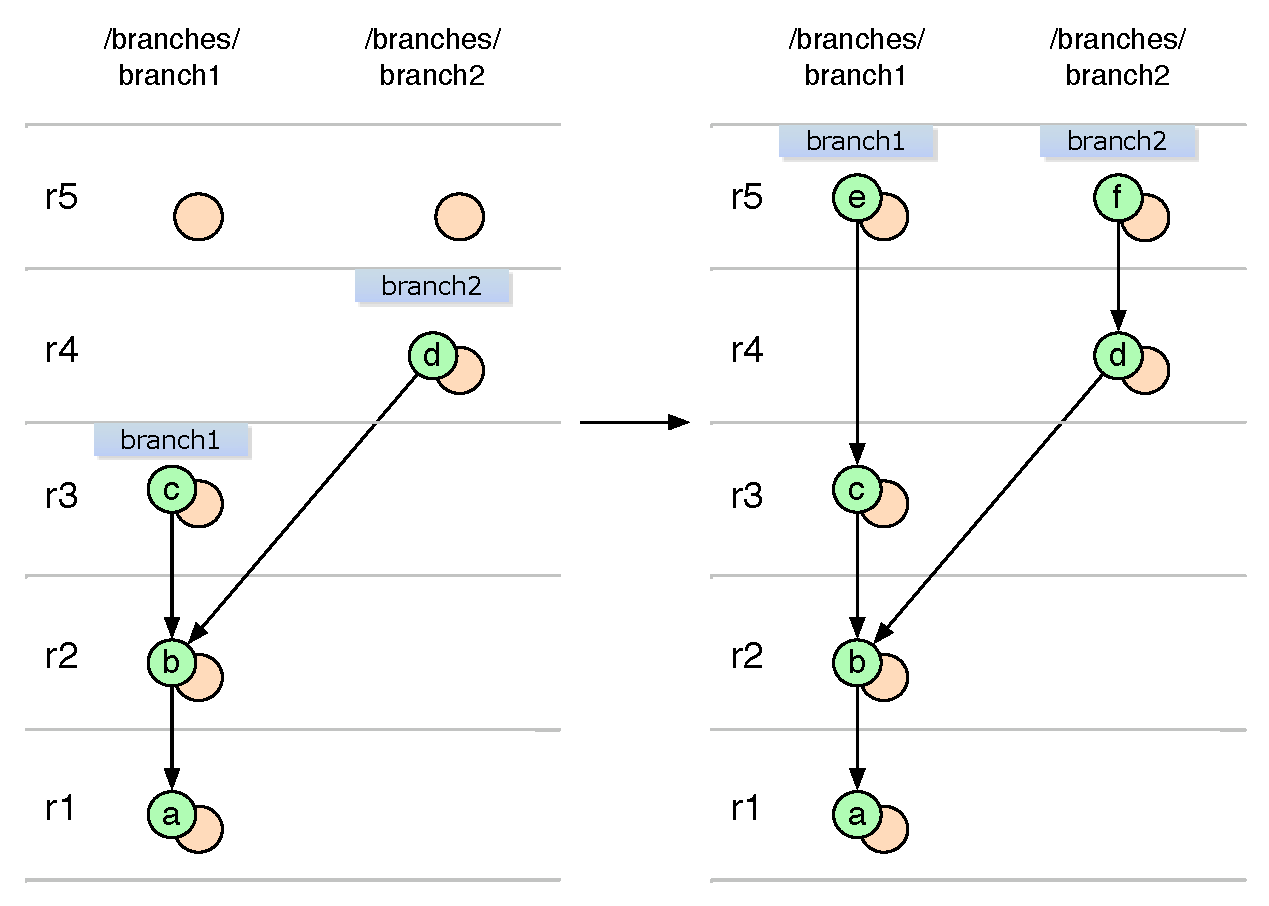
\includegraphics[width=\textwidth]{img/diagrams/double_branch_change_svn_to_git.pdf}%
\captionof{figure}{Revision modified two branches at once being translated to creation of two commits and updating corresponding branch references.}
\label{double_branch_change_svn_to_git}%
\end{center}

\subsubsection{Deletion}

1. Deletion of Subversion branch is always translated as deletion of corresponding Git branch as depicted at diagram \ref{branch_deletion_svn_to_git}. Single revision can remove an arbitrary number of branches, every corresponding Git branch is removed by Translator for that case.
\begin{center}
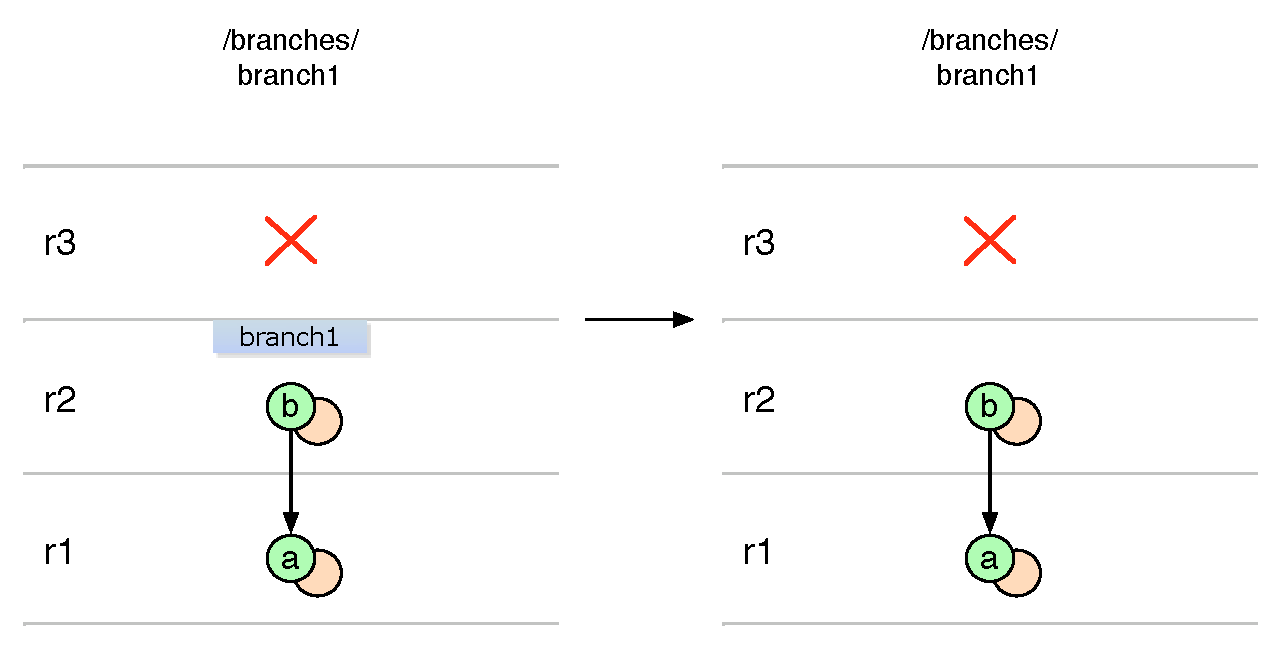
\includegraphics[width=\textwidth]{img/diagrams/branch_deletion_svn_to_git.pdf}%
\captionof{figure}{Deletion of Subversion branch being translated to Git branch removal.}
\label{branch_deletion_svn_to_git}%
\end{center}

2. And vice versa deletion of Git branch leads to deletion of corresponding branch at Subversion repository, see diagram \ref{branch_deletion_git_to_svn}. Multiple Git branches could be removed at once, as result Translator creates a single revision which removes every corresponding Subversion branch.
\begin{center}
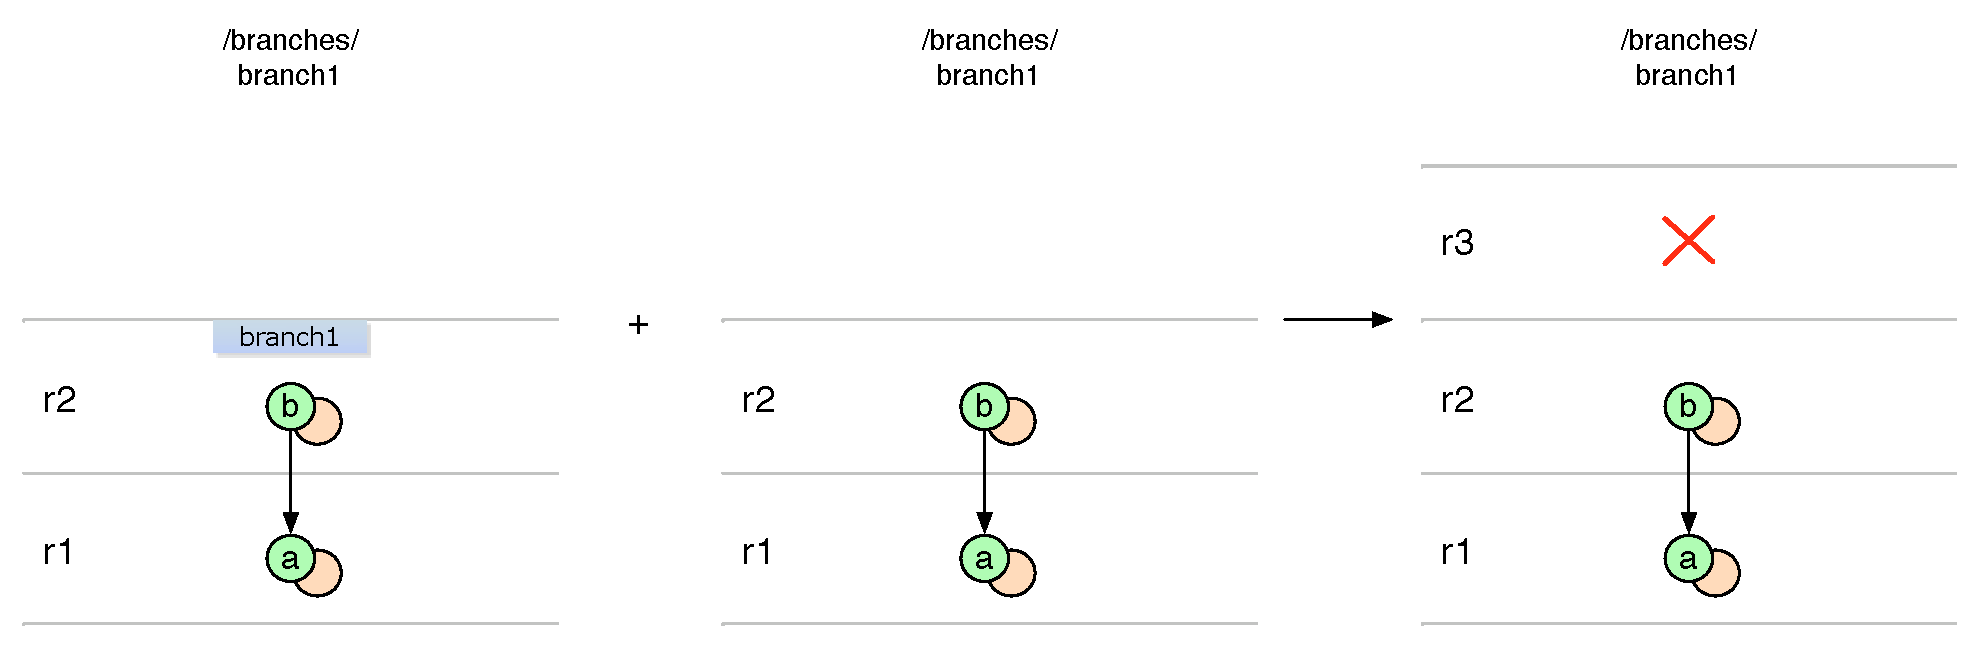
\includegraphics[width=\textwidth]{img/diagrams/branch_deletion_git_to_svn.pdf}%
\captionof{figure}{Deletion of Git branch being translated to Subversion branch removal.}
\label{branch_deletion_git_to_svn}%
\end{center}

\subsubsection{Replacement}

Subversion user is able to replace some branch by another, translation of that case is performed as shown on diagram \ref{branch_replacement_svn_to_git}.
\begin{center}
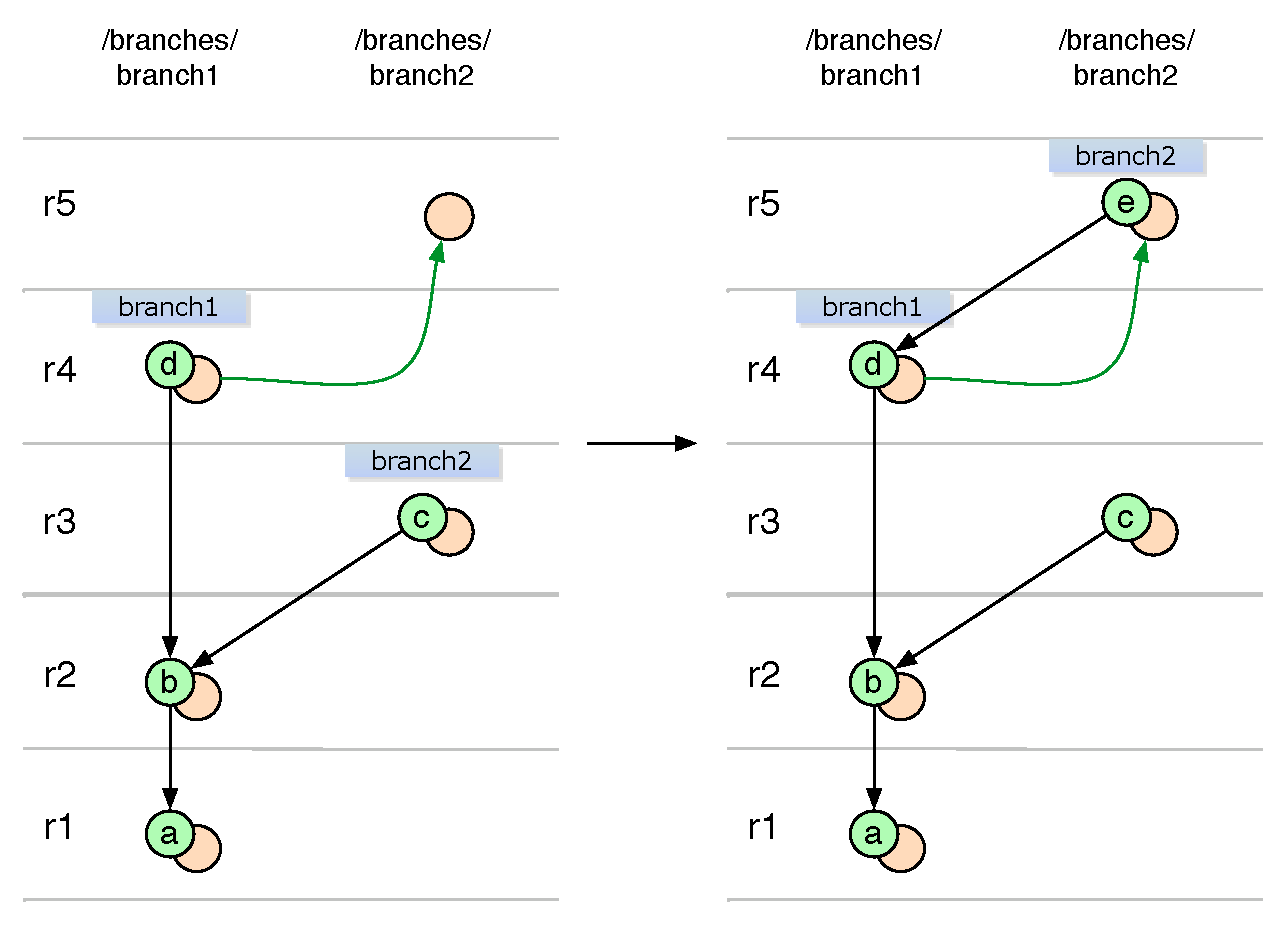
\includegraphics[width=\textwidth]{img/diagrams/branch_replacement_svn_to_git.pdf}%
\captionof{figure}{Replacement of Subversion branch being translated to replacement of Git branch.}
\label{branch_replacement_svn_to_git}%
\end{center}

Git user is able to reset any branch to any commit, that kind of changes is translated as shown at diagram \ref{branch_replacement_git_to_svn}.
\begin{center}
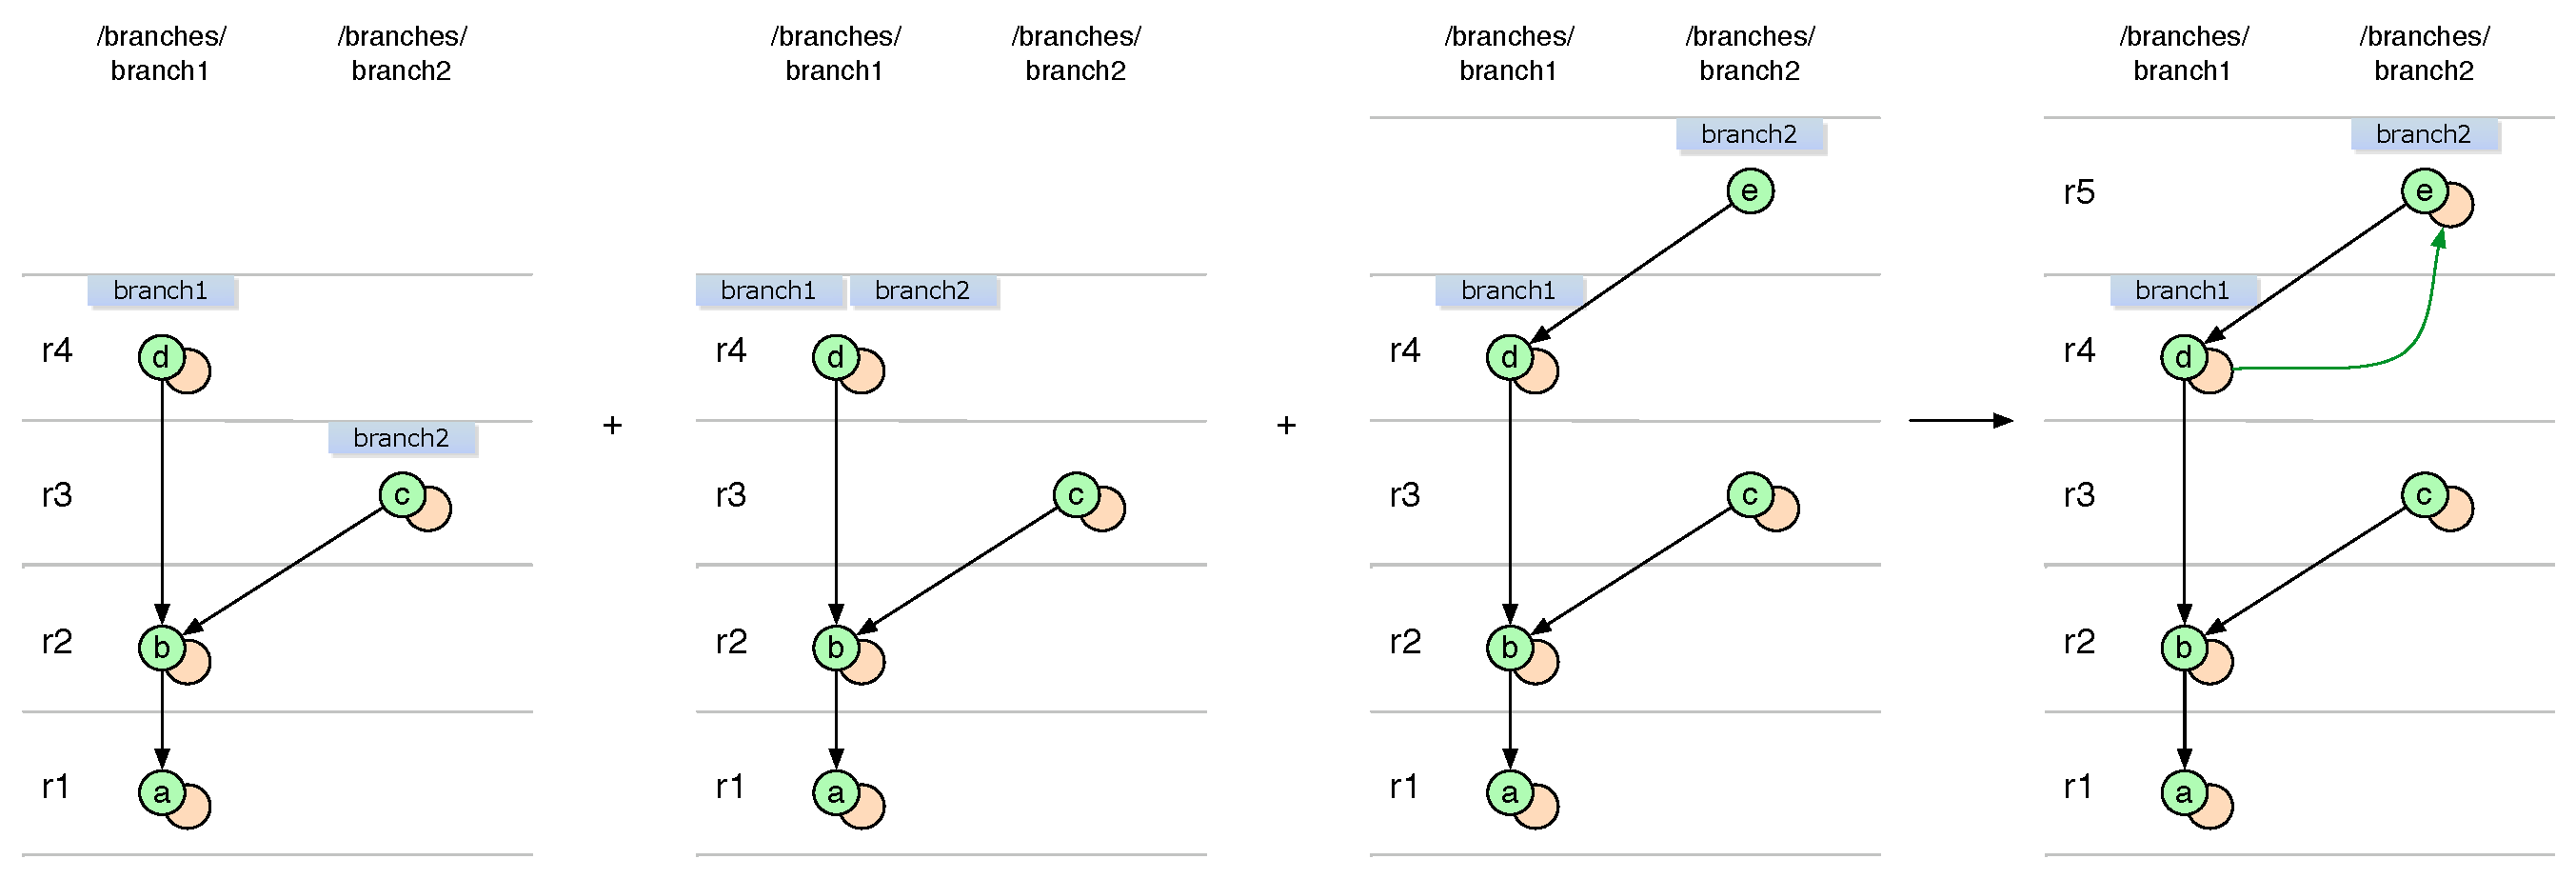
\includegraphics[width=\textwidth]{img/diagrams/branch_replacement_git_to_svn.pdf}%
\captionof{figure}{Replacement of Git branch being translated to replacement of Subversion branch.}
\label{branch_replacement_git_to_svn}%
\end{center}